% 无限深势阱中的高斯波包
% 无限深势阱|高斯波包|反射|积分|波函数

\pentry{无限深势阱\upref{ISW}, 高斯波包\upref{GausWP}}

我们下面来计算无限深势阱中一个高斯波包的运动. 定性来说, 波包会一边移动一边扩散(变宽变矮), 且在两个势阱壁之间来回反弹. 反弹的过程中会发生干涉.

结果如\autoref{wvISW_fig2} 和\autoref{wvISW_fig1}, 动画见\href{http://wuli.wiki/apps/wvISW.html}{百科互动演示}.

\begin{figure}[ht]
\centering
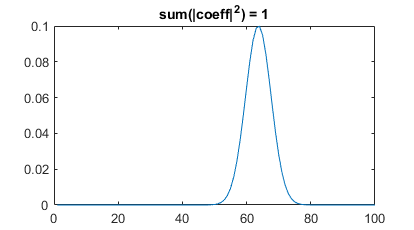
\includegraphics[width=8cm]{./figures/wvISW2.png}
\caption{束缚态概率分布, $x$ 轴为束缚态的 $n$, $y$ 轴为概率, 求和约等于 1} \label{wvISW_fig2}
\end{figure}

\begin{figure}[ht]
\centering
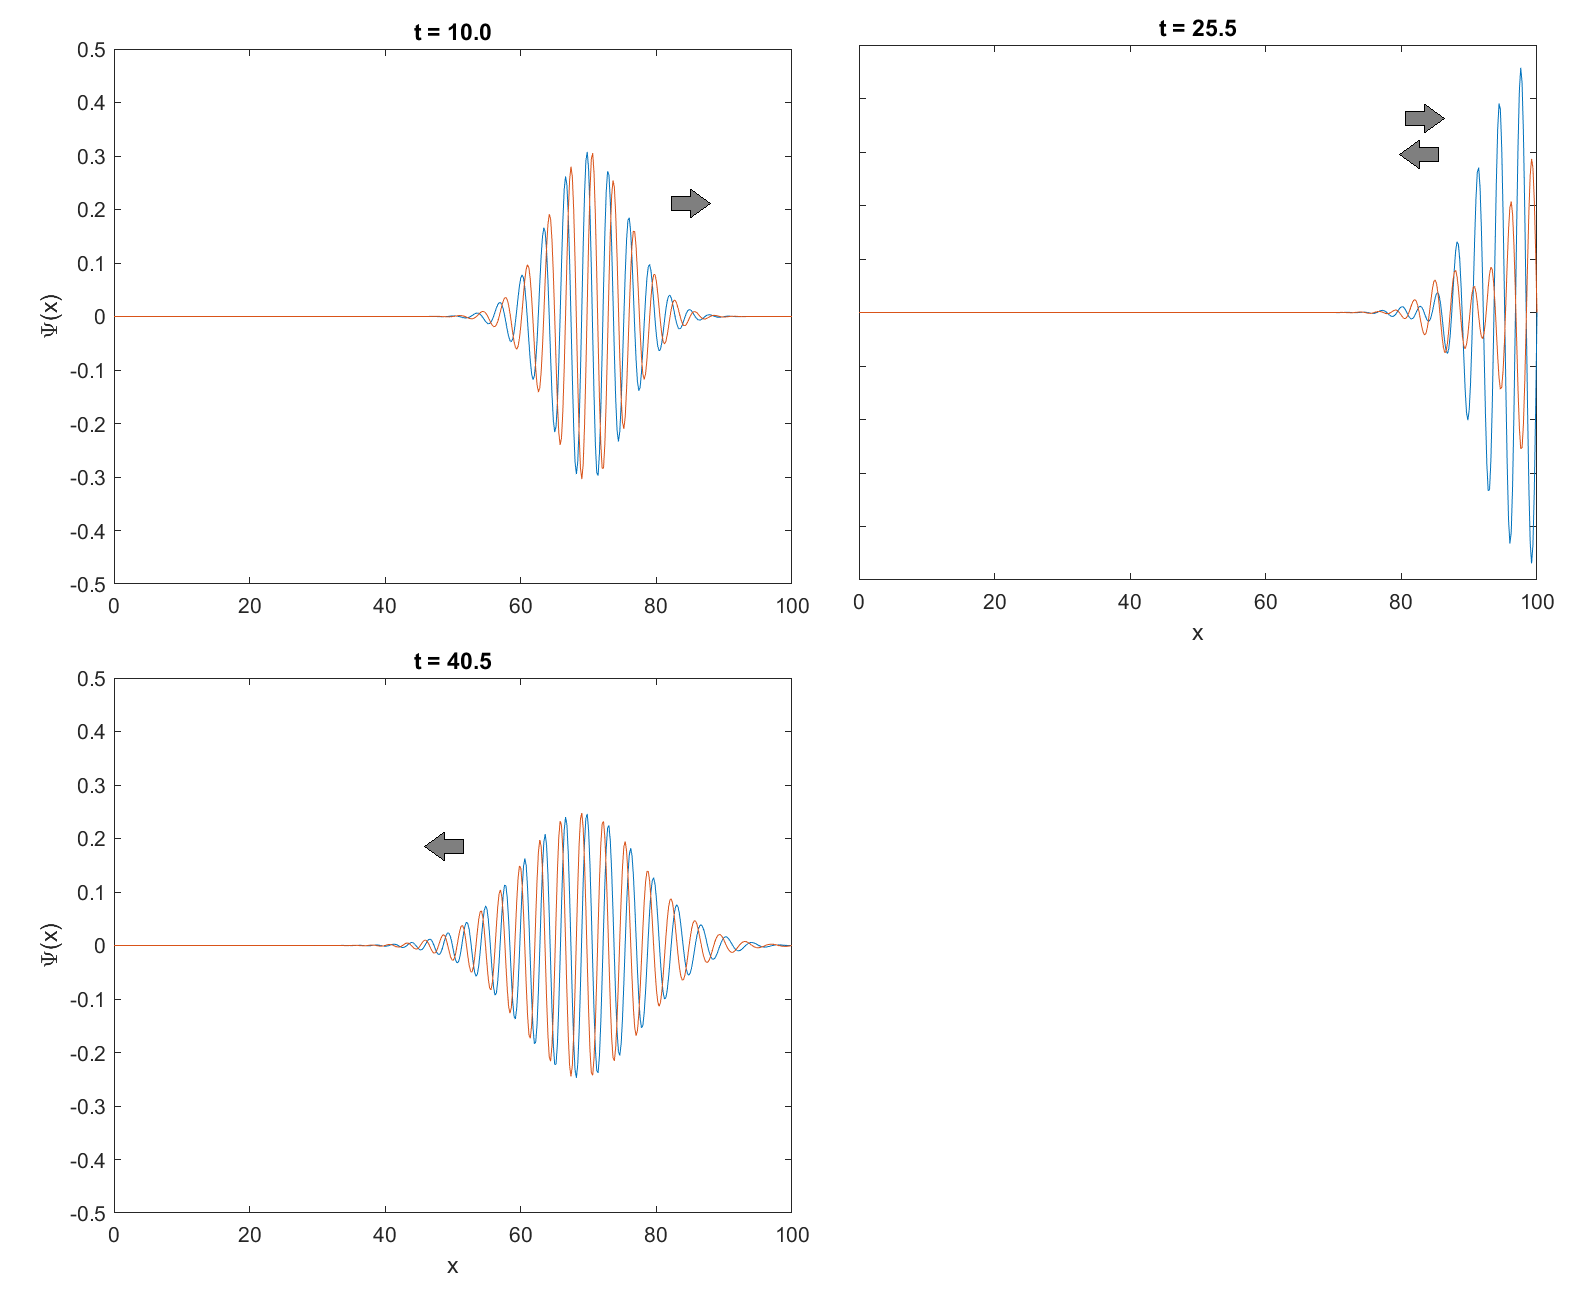
\includegraphics[width=15cm]{./figures/wvISW1.png}
\caption{波包遇到势阱壁后发生反弹, 过程中发生干涉} \label{wvISW_fig1}
\end{figure}

\subsection{算法}

本词条使用原子单位, 并假设粒子质量为 1. 假设无限深势阱的区间为 $[0, L]$, 能量的本征波函数(本征态)为(\autoref{ISW_eq1}\upref{ISW})
\begin{equation}
\psi _n(x) = \sqrt{\frac{2}{L}} \sin(k_n x)
\end{equation}
\begin{equation}
k_n = \frac{n\pi }{L}
\end{equation}
能量的本征值为
\begin{equation}
E_n = \frac{k_n^2}{2}
\end{equation}

初始时波函数为高斯波包(\autoref{GausWP_eq1}\upref{GausWP})
\begin{equation}
\psi (x,0) = \frac{1}{(2\pi \sigma _x ^2)^{1/4}} \E^{-(x - x_0)^2/(2\sigma _x)^2} \E^{\I k_0x}
\end{equation}

第一步是把初始波函数投影到能量本征态上
\begin{equation}\label{wvISW_eq1}
C_n = \int_0^L \psi _n^*(x) \psi (x,0) \dd{x}
= \int_0^L \sqrt{\frac{2}{L}} \sin(k_n x) \psi (x,0) \dd{x}
\end{equation}
那么接下来, 波函数的演化可以表示为
\begin{equation}\label{wvISW_eq2}
\psi (x,t) = \sum _i C_i \E^{-\I E_n t} \psi _n(x)
\end{equation}

若我们假设初始波包宽度足够小, 使得波函数在势阱外的函数值可以忽略不记, 则\autoref{wvISW_eq1} 的定积分可以拓展到无穷区间, 即傅里叶变换. 我们已经知道初始高斯波包(指数)傅里叶变换的结果为\autoref{GausWP_eq2}\upref{GausWP}
\begin{equation}
g(k) = \frac{1}{(2\pi \sigma _p^2)^{1/4}} \E^{-(k - k_0)^2/(2\sigma _k)^2} \E^{-\I x_0(k - k_0)}
\end{equation}
将正弦函数记为指数的形式为
\begin{equation}
\sqrt{\frac{2}{L}} \sin(k_n x) = \I \sqrt{\frac{\pi }{L}} \qty(\frac{\E^{-\I k_n x}}{\sqrt{2\pi }} - \frac{\E^{\I k_n x}}{\sqrt{2\pi }})
\end{equation}
所以\autoref{wvISW_eq1} 变为
\begin{equation}
C_n = \I \sqrt{\frac{\pi }{L}} [g(k_n) - g(-k_n)]
\end{equation}
带入\autoref{wvISW_eq2} 即可.

\subsection{Matlab 代码}

\Code{WpkISW}

